\documentclass[12pt, twoside]{article} 
\usepackage{graphicx}
\usepackage{setspace}

\begin{document}
\title{Capítulo 25, Exercício 44}
\author{Luiz Augusto Dembicki Fernandes GRR20202416}
\date{19/12/2022}
\maketitle

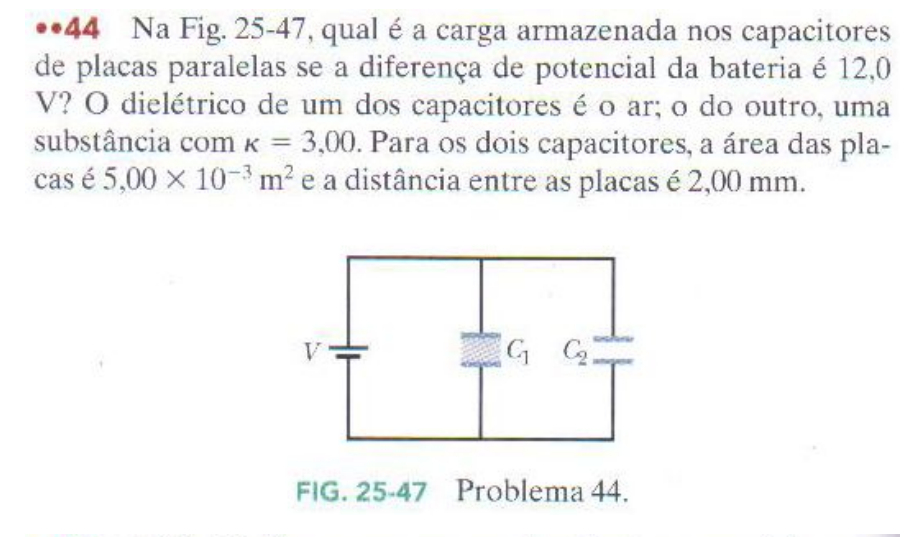
\includegraphics[width=11cm, height=8cm]{44.png}
\begin{doublespacing}
    

$ \Delta V = 12V \space ; k_{C1}= 3,00 \space ; A = 5,00\cdot 10^{-3} m^2 \space ; d = 2,00\cdot 10^{-3} m$ 

$ C_{0} = \frac{\varepsilon_0 A}{d} \space ; $  Como os capacitores estão em paralelo $ C_{eq} = C_1 + C_2 $ 

Calculando $ C_1 = k_{C_1} \frac{\varepsilon_0 A}{d} = 3,00 \cdot \frac{8,85 \cdot 10^{-12} \cdot 5,00\cdot 10^{-3} }{ 2,00\cdot 10^{-3}} \approx  6,6375 \cdot 10^{-11} F$

$ C_1 = k_{C_1} \frac{\varepsilon_0 A}{d} = 1 \cdot \frac{8,85 \cdot 10^{-12} \cdot 5,00\cdot 10^{-3} }{ 2,00\cdot 10^{-3}} \approx  2,2125 \cdot 10^{-11} F$

$ C_{eq} = C_1 + C_2  \space \to \space 2,2125 \cdot 10^{-11} + 6,6375 \cdot 10^{-11} \approx 8,85\cdot 10^{-11} F$ 

e utilizando $ C = \frac{ q }{ \Delta V } \to q = \Delta V \cdot C = 12,0V \cdot 8,85 \cdot 10^{-11}F \approx 1,062nC $

\end{doublespacing}
\end{document}